% !TeX root = ../main.tex
\chapter{System Test Plan}
\label{ch:system-test-plan}

\section{Introduction}

Once the detailed design and prototype construction have been done, then it is time to test the
entire power supply monitoring system to ensure that the hardware, embedded firmware,
user interface, and EPICS interface are working as expected. This chapter describes the test plan
that will be used in the evaluation of the prototype.

The purpose of testing is not just checking individual components of the design, but to demonstrate that the entire system is capable of monitoring all six power supply rails,
displaying measurements locally, sending measurements through the network and operating within
limits. Some parts of the system test will also be videotaped for use in the final project video.

\subsection{System Under Test}

The system under test is the completed six-channel power supply monitoring system
developed for this capstone project. The system monitors the following power rails:

\begin{itemize}
    \item \(+\SI{5}{\volt}{A}\)
    \item \(+\SI{5}{\volt}{B}\)
    \item \(+\SI{5}{\volt}\)
    \item \(-\SI{5}{\volt}\)
    \item \(+\SI{15}{\volt}\)
    \item \(-\SI{15}{\volt}\)
\end{itemize}

Each rail has its own separate voltage and current monitoring. The measurement
circuits are isolated from the communication channel on the Arduino side and are
connected to Arduino GIGA R1 WiFi. The Arduino has a local graphical display by
using GIGA Display Shield and Ethernet connection by a custom interface shield I've built.
The Ethernet connection works with EPICS Input/Output Controller (IOC), making
it possible to monitor the rails measurement and status remotely.

The testing of the system checks out the entire system but not each circuit block separately. This test involves the sensor circuits, isolation circuits, Arduino firmware, display, Ethernet connection, EPICS IOC, and related software
as one whole system.

\subsubsection{Test Objectives}

The primary objectives of the system test are to verify that:

\begin{enumerate}
    \item the complete system powers on and initializes without errors;
    \item all six power rails are identified and displayed correctly;
    \item the voltage measurement for each rail agrees with an external reference
    measurement within the specified system tolerance;
    \item the current measurement for each rail agrees with the applied load within
    the specified system tolerance;
    \item positive and negative supply rails are reported with the correct voltage
    polarity and current convention;
    \item measurements shown on the local display correspond with the values available
    through EPICS;
    \item voltage and current operating limits produce the appropriate status indication;
    \item user-configurable settings remain stored following a power cycle;
    \item Ethernet or IOC communication can be interrupted and restored without
    requiring a complete reprogramming of the monitor;
    \item measurement data can be recorded and used to generate a permanent test report;
    and
    \item the completed system can successfully perform the functions required for
    the final capstone demonstration.
\end{enumerate}

\subsection{Scope of Testing}

\subsubsection{Features to be Tested}

System testing will include the following functions:

\begin{itemize}
    \item system startup and initialization;
    \item detection and monitoring of all six power rails;
    \item voltage measurement;
    \item current measurement;
    \item measurement response to changes in load;
    \item correct handling of positive and negative rails;
    \item local GIGA Display operation;
    \item Ethernet communication;
    \item EPICS process-variable updates;
    \item voltage and current limit/status indications;
    \item storage and restoration of persistent settings;
    \item communication-loss recovery;
    \item repeated measurements to identify intermittent operation; and
    \item automatic recording and reporting of system test results.
\end{itemize}

\subsubsection{Features Not Included in This Test}

The system test is intended to verify the functional requirements of the prototype only. The following
tests are therefore outside the scope of this system-level test plan:

\begin{itemize}
    \item EMC testing;
    \item qualification tests for environmental temperature/humidity;
    \item qualification tests for vibrations or mechanical shock;
    \item qualification tests for life cycle/accelerated aging;
    \item destructive overvoltage tests; and
    \item destructive overcurrent tests.
\end{itemize}


\subsection{Test Equipment and Software}

The following equipment and software will be used during system testing:

\renewcommand{\arraystretch}{1.3}
\begin{longtable}{p{0.27\textwidth} p{0.63\textwidth}}
    \toprule
    \textbf{Equipment/Software} & \textbf{Purpose} \\
    \midrule
    \endfirsthead

    \toprule
    \textbf{Equipment/Software} & \textbf{Purpose} \\
    \midrule
    \endhead

    Power supply monitor prototype &
    Complete hardware and firmware system under test. \\

    DC bench supplies &
    Provide the six input rails required by the monitor. \\

    Rigol DL3021 electronic load &
    Provide programmable and repeatable loading of individual power rails. \\

    Computer running EPICS IOC &
    Receive voltage, current, and status information from the Arduino over Ethernet. \\

    Phoebus/EPICS display &
    Provide operator-level observation of process variables and system status. \\

    Python scripts &
    Control the electronic load, acquire EPICS values using PyEPICS, save raw
    test data, and automate portions of the test sequence. \\

    Ethernet network &
    Provide communication between the Arduino and EPICS IOC. \\

    \bottomrule
\end{longtable}

\subsection{Test Configuration}

During testing, the assembled power supply monitor will be operated in its normal
system configuration. All six monitored supplies will be connected to the appropriate
monitoring inputs. The Arduino, GIGA Display Shield, custom monitoring hardware,
and Ethernet interface will be powered and operating simultaneously.

For measurements involving the programmable electronic load, only the rail under
test will be connected to the electronic load. The remaining rails will remain
energized so that the monitor continues operating as a complete system, and may or may not be connected across resistive loads.

The electronic load measurement will provide the reference for both load voltage and current.

\subsection{System Acceptance Criteria}

The test is intended to establish whether the assembled prototype satisfies its
functional requirements. The following system-level acceptance criteria will be used.

\begin{longtable}{p{0.28\textwidth} p{0.62\textwidth}}
    \toprule
    \textbf{Parameter} & \textbf{Acceptance Criterion} \\
    \midrule
    \endfirsthead

    \toprule
    \textbf{Parameter} & \textbf{Acceptance Criterion} \\
    \midrule
    \endhead

    System startup &
    System initialization should not involve a firmware error or user action,
    and all six rails should be shown. \\

    Voltage measurement &
    The monitor reading should match the external reference voltage within
    \(\pm 2\%\) across the full tested operating range. \\

    Current measurement &
    Monitor reading should match the reference current within \(\pm 5\%\)
    across the full intended operating range. In addition, the uncertainty and
    resolution of the reference device should be considered at low currents. \\

    Positive/negative rail determination &
    Each measurement should use the correct polarity. The current in the negative
    channel should follow the sign convention used in the firmware. \\

    Display functionality &
    The display should show the proper identification of the rail, along with
    the rail voltage, current, and limits. \\

    EPICS operation &
    All process variables should communicate and report their status
    without errors in normal operations. \\

    Display and EPICS agreement &
    Local and remote readings should be identical to the same underlying
    measurement. Differences from rounding to integer in display are allowable. \\

    Limit status &
    Any programmed limit should change status as the corresponding measurement
    crosses the limit and return to the normal status upon the measurement
    returning to the allowable range. \\

    Persistent configuration &
    Any stored settings should be preserved after powering down and up the
    system. \\

    Network recovery &
    After the restoration of Ethernet communication, EPICS should continue to
    update without any firmware reprogramming. \\

    Test data &
    Each automatic test should yield a recorded raw-data file allowing for
    test results reconstruction. \\

    \bottomrule
\end{longtable}

The voltage and current accuracy requirements above are system-level requirements
rather than component-level accuracy specifications. They include the combined effects
of the sensor, shunt resistor, analog-to-digital conversion, calibration, wiring,
firmware calculations, and reference-instrument uncertainty.
\newpage
\subsection{System Test Matrix}

The system tests that are planned are listed in Table~\ref{tab:system-test-matrix} below.

\begin{Form}

    \begin{longtable}{
            p{0.065\textwidth}
            p{0.16\textwidth}
            p{0.29\textwidth}
            p{0.25\textwidth}
            p{0.105\textwidth}
        }
        \caption{System Level Test Matrix}
        \label{tab:system-test-matrix} \\

        \toprule
        \textbf{ID} &
        \textbf{Test} &
        \textbf{Method} &
        \textbf{Pass Criterion} &
        \textbf{Result} \\
        \midrule
        \endfirsthead

        \toprule
        \textbf{ID} &
        \textbf{Test} &
        \textbf{Method} &
        \textbf{Pass Criterion} &
        \textbf{Result} \\
        \midrule
        \endhead

        ST-01 &
        Power On and Initialization &
        Apply power to the entire system and check the operation of Arduino, the local
        display, the sensor channels and the network interface. &
        The system initializes properly, all six channels are operational. &
        \testresult{ST01} \\

        \addlinespace[0.4em]

        ST-02 &
        Rail Identification &
        Apply power to the six rails and correlate the displayed channel with the
        corresponding input physical connection. &
        The correct rail identification with the right polarity occurs. &
        \testresult{ST02} \\

        \addlinespace[0.4em]

        ST-03 &
        Voltage Accuracy &
        Measure each rail using a DMM or the E-Load and compare the reference value
        with the local and EPICS values at different operating points. &
        The error is within the specified voltage tolerance. &
        \testresult{ST03} \\

        \addlinespace[0.4em]

        ST-04 &
        Current Accuracy &
        Apply different loads to each rail using the programmable electronic load and
        compare the reference current with the monitor measurement. &
        The error is within the specified current tolerance. &
        \testresult{ST04} \\

        \addlinespace[0.4em]

        ST-05 &
        Dynamic Load Response &
        Change the current of the electronic load while monitoring the local display
        and EPICS values. &
        The current and voltage readings change accordingly to the load change. &
        \testresult{ST05} \\

        \addlinespace[0.4em]

        ST-06 &
        Local Display &
        Monitor voltage, current, rail identification and status of all channels. &
        All necessary information is visible and correlates with the connected rail. &
        \testresult{ST06} \\

        \addlinespace[0.4em]

        ST-07 &
        EPICS Communications &
        Run the IOC and check all voltage, current and status process variables. &
        All necessary process variables are connected and updated properly. &
        \testresult{ST07} \\

        \addlinespace[0.4em]

        ST-08 &
        Limit / Alarm Operation &
        Set a limit and change the current of the electronic load or supply until the
        measured value reaches this limit. &
        The proper limit indication is created and then is cleared when the value is
        inside the limits. &
        \testresult{ST08} \\

        \addlinespace[0.4em]

        ST-09 &
        Persistent Settings &
        Change some settings, cycle system power and check the value after the
        power-up. &
        The stored value is restored properly. &
        \testresult{ST09} \\

        \addlinespace[0.4em]

        ST-10 &
        Communication Recovery &
        Disconnect Ethernet while the system is running and reconnect the network and
        monitor the IOC. &
        Monitoring on the local machine continues and communication recovers. &
        \testresult{ST10} \\

        \addlinespace[0.4em]

        ST-11 &
        Repeatability &
        Make repeated measurements at selected points, including after power cycle. &
        Measurement remains within the specified acceptance limits with no
        intermittent failures of the channels. &
        \testresult{ST11} \\

        \addlinespace[0.4em]

        ST-12 &
        End-To-End Demonstration &
        Run all parts of the system and demonstrate the operation of local and remote
        monitoring by changing the load on the selected channel. &
        All hardware, firmware, display, network, IOC and test software run
        cooperatively with no system level failure. &
        \testresult{ST12} \\

        \bottomrule
    \end{longtable}

\end{Form}
\newpage
\subsection{Detailed Test Procedures}

\subsubsection{ST-01: Power-On and Initialization}

\begin{enumerate}
    \item Inspect all power, sensor, display, and Ethernet connections.
    \item Verify that the electronic load is disabled.
    \item Energize the required monitored power supplies.
    \item Apply power to the Arduino and monitoring electronics.
    \item Observe the Arduino startup sequence.
    \item Confirm that the GIGA Display initializes.
    \item Confirm that all six expected rail channels are displayed.
    \item Start or verify operation of the EPICS IOC.
    \item Verify that the IOC establishes communication with the monitor.
    \item Record any startup errors or unexpected behavior.
\end{enumerate}

The test passes when the complete system reaches its normal operating state without
manual recovery, all six rail channels are present, and network communication can
be established.

\subsubsection{ST-03 and ST-04: Voltage and Current Measurement}

Voltage and current accuracy testing will be performed for each of the six rails.
Testing will be automated where practical to improve repeatability and preserve the
raw test data.

For each selected rail:

\begin{enumerate}
    \item Select the rail to be tested in the Python test program.
    \item Verify the physical connection of the rail and electronic load.
    \item Connect the DMM directly across the rail.
    \item Set the electronic load to its initial test condition with the input disabled.
    \item Enable the load.
    \item Allow the readings to stabilize.
    \item Record the DMM or E-Load reference voltage.
    \item Record the electronic-load reference current.
    \item Acquire the corresponding EPICS voltage and current values using PyEPICS.
    \item Calculate the voltage and current measurement errors.
    \item Repeat the measurement at several loads distributed throughout the intended
    operating range of the rail.
    \item Disable the load before changing connections.
    \item Save all raw measurements to the test-data file.
\end{enumerate}

Voltage error will be calculated as

\begin{equation}
    \text{Voltage Error (\%)} =
    \frac{V_{\text{monitor}}-V_{\text{reference}}}
    {|V_{\text{reference}}|}
    \times 100.
\end{equation}

Current error will be calculated as

\begin{equation}
    \text{Current Error (\%)} =
    \frac{I_{\text{monitor}}-I_{\text{reference}}}
    {|I_{\text{reference}}|}
    \times 100.
\end{equation}

Absolute error will also be retained in the raw data. This is particularly important
for low-current measurements where percentage error alone can become misleading.

A rail passes when each required measurement point remains within the specified
acceptance criteria. If a point fails, the rail may be retested after the cause of
the failure is investigated. Original failed data will not be deleted when a retest
is performed.

\subsubsection{ST-07: EPICS Communication Test}

\begin{enumerate}
    \item Power the complete monitor and connect it to the Ethernet network.
    \item Start the EPICS IOC.
    \item Verify that the IOC connects to the Arduino TCP server.
    \item Observe the voltage and current process variables for all six rails.
    \item Compare the EPICS values with the local display.
    \item Change the load on a selected rail.
    \item Verify that the corresponding EPICS voltage and current values update.
    \item Repeat the load change on at least one positive and one negative rail.
\end{enumerate}

The test passes when the required process variables remain connected, values change
in response to the physical system, and EPICS and local-display values agree within
their displayed resolution.

\subsubsection{ST-08: Limit and Status Test}

\begin{enumerate}
    \item Select a rail for testing.
    \item Record the existing voltage and current limit settings.
    \item Configure a test limit that can be crossed safely without exceeding the
    electrical rating of the hardware.
    \item Operate the rail below the limit and verify that normal status is displayed.
    \item Increase or decrease the applied load until the selected threshold is crossed.
    \item Verify the local status indication.
    \item Verify the corresponding EPICS status.
    \item Return the measurement to the normal operating range.
    \item Verify that the status returns to normal.
    \item Restore the original limit setting.
\end{enumerate}

No test limit shall require the monitored supply, sensor, wiring, or electronic load
to be operated outside its rated limits.

\subsubsection{ST-09: Persistent Settings Test}

\begin{enumerate}
    \item Change one or more user-adjustable system settings to known values.
    \item Verify that the settings are accepted by the firmware.
    \item Remove power from the Arduino and monitor electronics.
    \item Wait several seconds.
    \item Restore power.
    \item Allow the firmware to complete initialization.
    \item Read the previously modified settings.
    \item Compare the restored values with the values stored before power removal.
\end{enumerate}

The test passes when all settings intended to be persistent are restored without
requiring Ethernet communication or manual re-entry.

\subsubsection{ST-10: Communication-Loss and Recovery Test}

\begin{enumerate}
    \item Establish normal communication between the monitor and IOC.
    \item Verify that EPICS values are updating.
    \item Disconnect the Ethernet cable.
    \item Verify that local monitoring and the GIGA Display continue operating.
    \item Observe the IOC response to the communication failure.
    \item Reconnect the Ethernet cable.
    \item Verify that communication is re-established.
    \item Confirm that the process variables resume updating with valid values.
\end{enumerate}

The system passes if the loss of Ethernet communication does not prevent local
operation and normal EPICS communications resume after the network connection is
restored.

\subsection{Automated Test Data Collection}

A Python test application will be used for measurement testing. The application
interfaces with the Rigol DL3021 programmable electronic load and the EPICS IOC.
EPICS Channel Access is performed using the PyEPICS library.

The test operator may select an individual power rail instead of being required to
test all six rails in a single session. This permits channels to be tested or
retested at different times while retaining all results as part of the same system
test campaign.

For each test point, the following information will be retained when applicable:

\begin{itemize}
    \item test date and time;
    \item rail identification;
    \item test iteration;
    \item electronic-load operating mode;
    \item programmed load value;
    \item reference voltage;
    \item reference current;
    \item EPICS voltage measurement;
    \item EPICS current measurement;
    \item absolute voltage error;
    \item percentage voltage error;
    \item absolute current error;
    \item percentage current error;
    \item applicable limits;
    \item test result; and
    \item operator notes.
\end{itemize}

Raw data will be preserved independently from the final report so that the report
can be regenerated without repeating the physical test. After the required tests
have been completed, the saved data will be processed using ReportLab to produce
a final test report containing the recorded values and pass/fail results.

\subsection{Test Execution and Result Classification}

Each test will be assigned one of the following results:

\begin{description}
    \item[PASS:] The test was completed and all applicable acceptance criteria were met.
    \item[FAIL:] The test was completed but one or more acceptance criteria were not met.
    \item[INCOMPLETE:] The test could not be completed because of an unrelated equipment,
    software, or setup problem.
    \item[RETEST:] A previously failed or incomplete test was repeated following a
    corrective action.
\end{description}

A failed test will not be deleted or overwritten following corrective action. The
original result and subsequent retest will both be retained to provide traceability
of the development process.

\subsection{Suspension and Resumption Criteria}

Testing will be immediately suspended if any of the following conditions occur:

\begin{itemize}
    \item unexpected overheating of a component or conductor;
    \item evidence of a short circuit or incorrect wiring;
    \item operation outside the rated voltage or current of the test equipment;
    \item unstable or uncontrolled power-supply output;
    \item a firmware condition that could apply an unintended load;
    \item loss of isolation where isolation is required; or
    \item any condition that could damage the prototype or test equipment.
\end{itemize}

Testing may resume after the cause has been identified, corrective action has been
completed, and the affected portion of the system has been inspected or verified
before power is reapplied.

\subsection{Test Responsibilities}

As the designer and developer of the capstone project, Mike Capotosto will serve as the
primary test operator. Responsibilities include:

\begin{itemize}
    \item preparing and inspecting the test setup;
    \item configuring the test equipment;
    \item executing each test procedure;
    \item recording results;
    \item identifying and documenting failures;
    \item making required corrections;
    \item performing retests;
    \item maintaining the raw test data; and
    \item preparing the final test report and demonstration.
\end{itemize}

Where practical, automated data acquisition will be used to reduce transcription
errors and improve repeatability.

\subsection{Testing Risks and Contingencies}

Several risks may affect system testing. Improper electronic-load connections,
particularly when testing the negative supply rails, could damage the electronic
load or power supply. Connections will therefore be verified before the load input
is enabled.

Network problems could also produce an apparent measurement failure when the actual
sensor hardware is operating correctly. Local display values and direct instrument
measurements will be used to distinguish a network or IOC problem from a hardware
measurement problem.

A failed sensor channel could prevent the complete six-channel system test from
being performed. Because the test software allows individual rail selection, completed
channel data can be retained while the affected channel is repaired and subsequently
retested.

Finally, automatic test software itself could introduce an error in the recorded
results. Critical results will therefore be compared with the front-panel readings
of the electronic load, local display, and EPICS interface during
initial testing to confirm correct operation of the automation.

\subsection{Test Deliverables}

The completed system test will produce the following deliverables:

\begin{itemize}
    \item this system test plan;
    \item saved raw test data;
    \item automatically generated test report;
    \item documentation of failed tests and corrective actions;
    \item results of any required retests;
    \item photographs of the final test configuration; and
    \item video footage demonstrating selected system-level tests.
\end{itemize}

\subsection{Test Completion Criteria}

System-level testing will be considered complete when:

\begin{enumerate}
    \item every test identified in Table~\ref{tab:system-test-matrix} has been executed;
    \item each of the six rail channels has completed voltage and current verification;
    \item all critical functional tests have received a PASS result;
    \item any failed tests have been documented and either corrected and retested or
    identified as known limitations;
    \item raw test data has been preserved;
    \item the final test report has been generated
\end{enumerate}

Successful completion of this test plan will demonstrate that the individual hardware
and software portions developed throughout the project operate together as a complete
power supply monitoring system.

\subsection{Test Plan and Results}
\label{sec:part-a-test-results}

The test plan developed in in the previous chapter was performed after completion of hardware bring-up, firmware development, local display integration, Ethernet communications, and EPICS IOC integration. Testing was done for the whole assembled system instead of the individual circuit blocks in order to assess the interactions between the sensor hardware, Arduino controller, firmware, local display, Ethernet communications, EPICS IOC, and test software.

The final test produced the automated PDF system test report containing acceptance criteria, overall test matrix, rail-by-rail measurement results, error plots, operator observations, detailed system test checklist, completion criteria, and engineering justification for the selected tolerances. The complete generated report is attached at the end of Part A.

\subsubsection{Test Execution}

Tests were conducted on each of the six monitored power supply rails:

\begin{itemize}
    \item +5VA,
    \item +5VB,
    \item +5~V,
    \item $-$5~V,
    \item +15~V, and
    \item $-$15~V.
\end{itemize}

A Rigol programmable electronic load was used to set multiple load cases on each rail. During each test point, the external reference voltage and current were compared with the corresponding measurements reported by the EPICS IOC. The local GIGA display was also observed to check rail identity, polarity, measurements updates, limits state and communication state.

The +5VA and +5VB channels were tested at approximately 0~A, 1~A, and 2~A. The other +5~V, $-$5~V, +15~V, and $-$15~V channels were tested at approximately 0~A, 0.5~A, and 1~A. The result was multiple operating points for every monitored rail instead of checking the system under a single load.

The Python test software automated the acquisition of the EPICS values, measurement error calculation, application of acceptance limits, data saving and generation of the final PDF report. When operator observation was required, such as the verification of the information displayed on the local display, the result was recorded in the system test checklist.

\subsubsection{Acceptance Criteria}

The acceptance criteria formulated in the previous chapter were kept for the final system test. The main electrical acceptance criteria were:

\begin{itemize}
    \item The IOC voltage measurements must agree with the external reference within $\pm2\%$ across the whole test range.
    \item The IOC current measurements must agree with the external reference within $\pm5\%$ across the whole intended range.
    \item For low current values, the bigger of the percentage tolerance and absolute error floor is used. The absolute floor is 25~mA for the 39~m$\Omega$ channels and 20~mA for the 50~m$\Omega$ channels.
    \item Positive and negative rail voltages must be represented correctly in terms of polarity.
    \item The local-display and EPICS values must represent the same underlying measurement within the display resolution and rounding.
    \item Programmable voltage and current limits must work correctly in terms of assertion and de-assertion.
    \item Persistent settings must survive the removal and restoration of the controller power.
    \item Local monitoring must operate during network interruption and the EPICS communication must be restored after Ethernet recovery.
\end{itemize}

These criteria provided the measurable limits by which the completed prototype could be evaluated instead of the subjective judgment that the system appeared to be working.

\subsubsection{System Test Results}

The system test of the completed system produced the overall result of \textbf{PASS}. All six rail measurement tests passed, and each of the twelve system level tests formulated in Chapter 6 also passed.

Table~\ref{tab:system-test-results} summarizes the final system test disposition.

\begin{table}[htbp]
    \centering
    \caption{Final system test results.}
    \label{tab:system-test-results}
    \begin{tabular}{clc}
        \hline
        \textbf{Test ID} & \textbf{Test} & \textbf{Result} \\
        \hline
        ST-01 & Power On and Initialization & PASS \\
        ST-02 & Rail Identification & PASS \\
        ST-03 & Voltage Accuracy & PASS \\
        ST-04 & Current Accuracy & PASS \\
        ST-05 & Dynamic Load Response & PASS \\
        ST-06 & Local Display & PASS \\
        ST-07 & EPICS Communications & PASS \\
        ST-08 & Limit / Alarm Operation & PASS \\
        ST-09 & Persistent Settings & PASS \\
        ST-10 & Communication Recovery & PASS \\
        ST-11 & Repeatability & PASS \\
        ST-12 & End-To-End Demonstration & PASS \\
        \hline
    \end{tabular}
\end{table}

Also, the latest accepted attempt for each individual rail passed, as summarized in Table~\ref{tab:rail-results}.

\begin{table}[htbp]
    \centering
    \caption{Final rail measurement results.}
    \label{tab:rail-results}
    \begin{tabular}{ccc}
        \hline
        \textbf{Rail} & \textbf{IOC Channel} & \textbf{Result} \\
        \hline
        +5VA  & 5VA  & PASS \\
        +5VB  & 5VB  & PASS \\
        +5~V  & P5V  & PASS \\
        $-$5~V  & M5V  & PASS \\
        +15~V & P15V & PASS \\
        $-$15~V & M15V & PASS \\
        \hline
    \end{tabular}
\end{table}

All required voltage samples satisfied the system-level voltage accuracy criterion, and all required current samples satisfied the current accuracy criterion, including the low current absolute tolerance when applicable. Both negative voltage channels reported the correct negative voltage polarity while preserving the positive current magnitude convention used by the firmware.

Dynamic load testing also passed on all six channels. The changes in electronic load current were reflected on the local display and on the corresponding EPICS process variables, and none of the channels became unresponsive during the load sweeps.

Local display testing confirmed that all six channel identifications, voltage values, current values, programmed limits, status indication, and communication information were visible and corresponded to the appropriate physical rail. All local display observations recorded during the test passed for every monitored channel.

EPICS communication testing confirmed that the IOC connected to the Arduino TCP server and that the required voltage and current process variables for all six rails were connected and updated. The load changes were observed by EPICS for both positive and negative channels, confirming the proper operation of the complete measurement and communication chain.

Limit testing confirmed that the system reacted correctly when the applied measurement crossed the programmed threshold. Both the local display and the EPICS status changed when the threshold was exceeded and returned to normal when the measurement came back inside the configured limits.

Persistent settings testing was performed by changing known user-adjustable settings, removing power from the monitoring electronics, restoring power, and comparing the recovered values with the values stored prior to the power cycling. The stored values were recovered correctly.

Communication recovery testing was performed by interrupting Ethernet communication while the monitor was running. The local GIGA display continued to operate during the interruption. After Ethernet was restored, the communication with the IOC was recovered without firmware reprogramming and the EPICS process variables started to update again with the valid values.

Repeatability testing was also passed. The measurements repeated at selected operating points, including after the power cycle, were within the established acceptance limits, and no intermittent sensor or communication problems were observed.

Finally, the end-to-end demonstration confirmed simultaneous operation of the complete hardware, firmware, local display, network interface, EPICS IOC, Phoebus interface and automated test software. The change of the load on the monitored channel produced the expected result locally and remotely without system-level problems.

\subsubsection{Conclusions and Results}

The final test results confirm that the completed prototype satisfied the main functional and measurement requirements established for the project. All twelve system level tests passed and all six monitoring channels passed their final voltage and current verification.

The voltage and current tests are especially important since they give the quantitative proof that the monitor implements its intended measurement function. The testing was performed at multiple operating points on each channel instead of the single nominal load case. This gives the higher confidence that the measurement system works properly across the intended range of loads.

The test results also confirmed the functions that cannot be confirmed by measurement accuracy alone. Correct rail identification and polarity were confirmed, including the two negative voltage channels. The local graphical interface and EPICS interface displayed the same underlying information, programmable limits worked correctly, persistent settings were recovered from the storage, and the network communication was restored after the intentional interruption.

The conclusion regarding the operation of the system in the broad range of temperature, electromagnetic compatibility, vibration, mechanical shock, accelerated aging, and destructive fault conditions cannot be made since these qualification tests were intentionally excluded from the system test plan. The additional measurements are needed to make claims regarding performance under those conditions.

Some of the problems discovered during the board bring-up were fixed before the final system test. They included the SDA polarity problem in the isolated I\textsuperscript{2}C interface, pull-up and signal state problems, and startup sequencing problems. The successful final acceptance test confirms that the corrective modifications were effective and that these earlier development problems did not prevent the completed prototype from passing the final system test.

\subsubsection{Recommendations and Improvement Opportunities}

Despite the fact that the completed system satisfied the acceptance criteria, some improvements are recommended for the future PCB revision.

The most important hardware improvement is the incorporation of the SDA polarity fix directly in the PCB design. The prototype required the SN74LVC2G04 inverter to correct the SDA signal polarity after the originally installed LTC2945 device variant turned out to be incompatible with the intended isolation interface. The future revision should use the correct LTC2945 variant throughout the design or incorporate the required inversion directly in the schematic and PCB.

All required I\textsuperscript{2}C pull-up resistors and defined logic states should also be incorporated directly in the next PCB revision. It will eliminate the prototype modification and improve the repeatability of assembly and startup.

The firmware initialization can also be made more tolerant of arbitrary power-up sequencing. During the development, the communication could be failed when the controller tried to initialize the sensor before the corresponding isolated rail circuitry was powered. The future firmware revision could periodically retry the unavailable sensors so that the communication is established automatically when the monitored rail is powered.

The per-channel measurement calibration is another potential improvement. The present system calculates the current using the configured current sense resistance. The measurement of the actual resistance or the determination of the calibration factor against the external reference will allow the individual gain correction to be stored for each channel. It will help to reduce the systematic errors caused by the shunt tolerance and allow tighter acceptance limits if the improved measurement accuracy is required.

The additional environmental characterization is also useful if the design is going to be developed beyond the capstone prototype. The testing at multiple ambient temperatures can be used to determine whether the temperature affects the measurement accuracy. EMC testing can determine the susceptibility to and generation of the electromagnetic interference. The long duration testing can be used to detect the intermittent communication, thermal, network or firmware problems that might not occur during the shorter acceptance test.

The automated test system should be retained for the future revisions. Since the raw measurements are saved separately from the report generation, the future hardware or firmware revisions can be tested using the same acceptance procedure and direct comparison between the revisions is possible.

These recommendations represent the refinements in reliability, manufacturability, calibration and qualification and not the changes to the basic architecture. The successful final test proves that the overall system concept is suitable for the further development.

\subsubsection{Generated System Test Report}
\label{sec:generated-test-report}

The automated System Test Report generated from the final accepted test data is attached below as the permanent part of the project test record. The report contains the detailed rail-by-rail measurements, measurement error plots, system test checklist, acceptance results, and engineering justification for the selected tolerances.

\clearpage

% Requires \usepackage{pdfpages} in the document preamble.
% Change the path below if the PDF is stored in another directory.
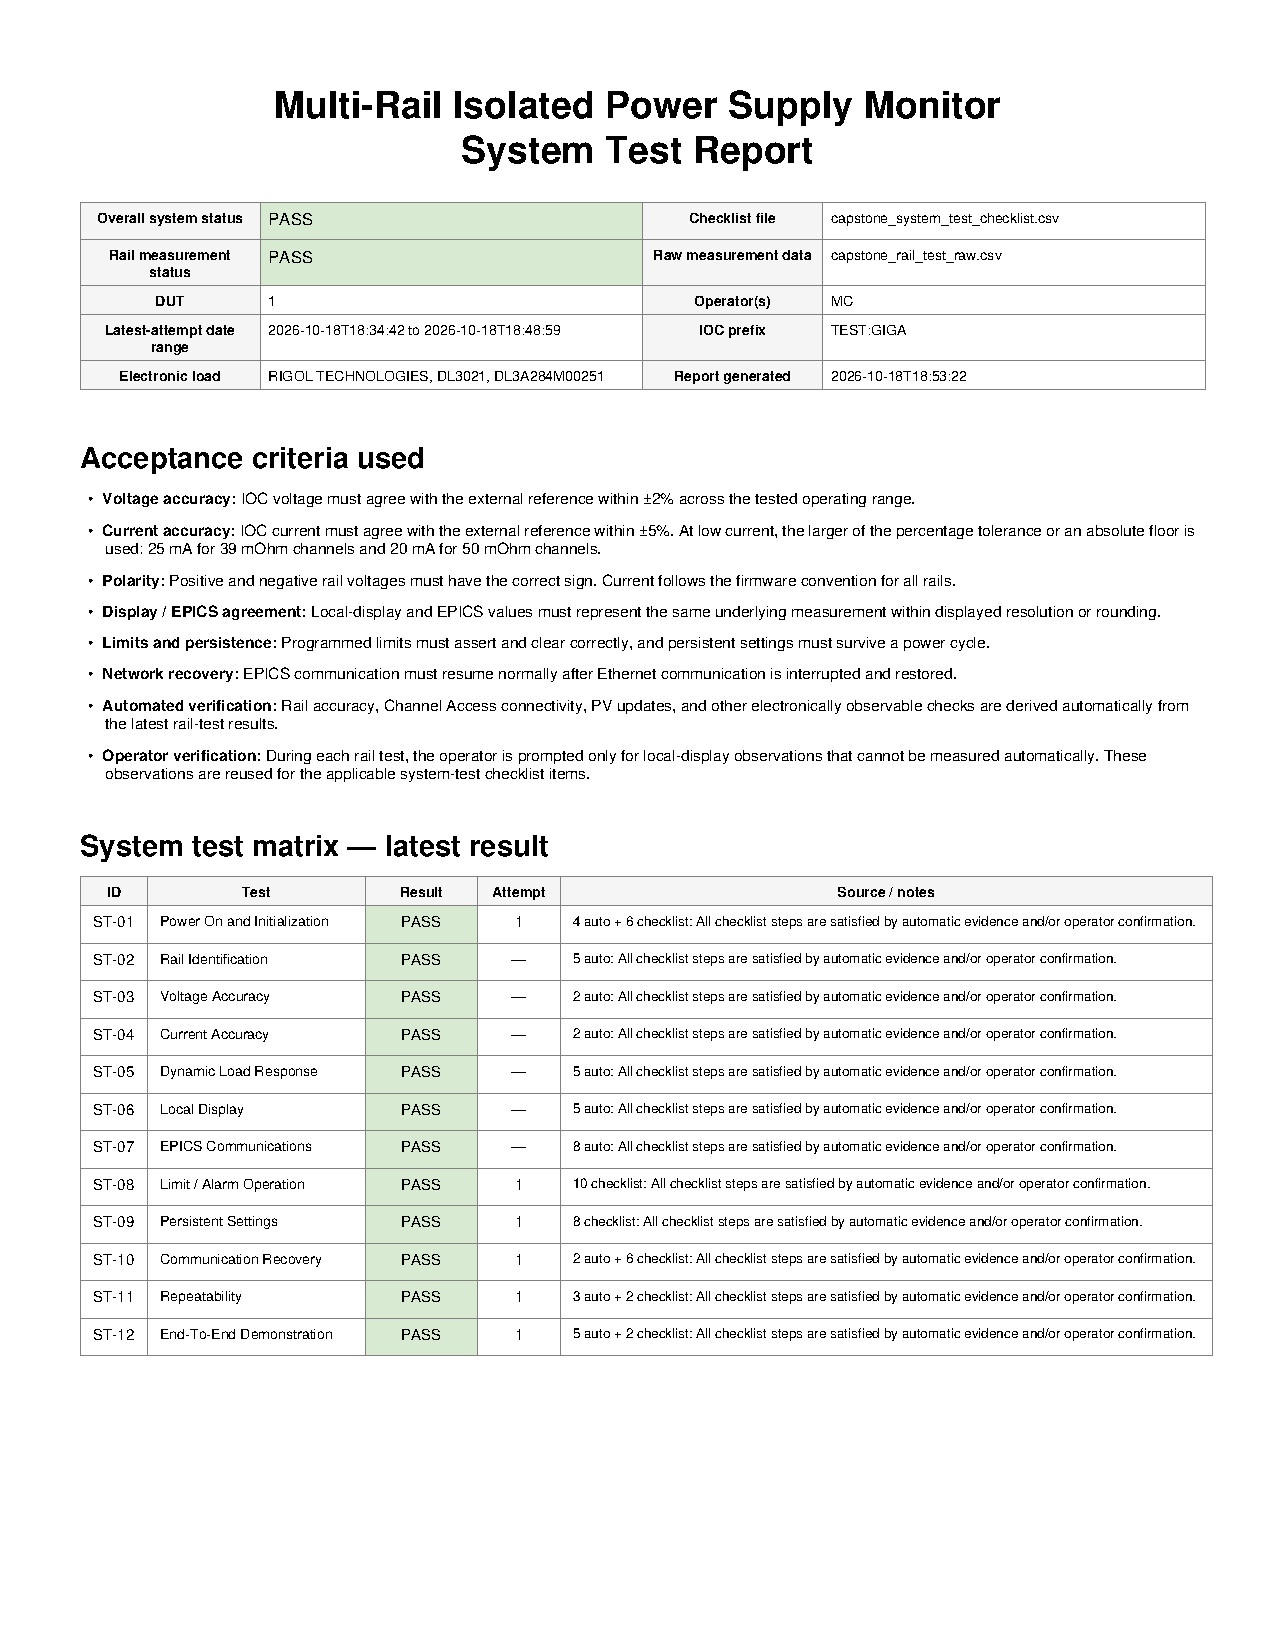
\includepdf[
pages=-,
pagecommand={\thispagestyle{plain}},
fitpaper=true
]{Pictures/capstone_rail_test_report_20261018_185322.pdf}